\documentclass[border=10pt]{standalone}

\usepackage{tikz}
\usepackage{tikzsymbols}
\usetikzlibrary{calc,patterns,shapes.geometric}

\def\centerarc[#1](#2)(#3:#4:#5){\draw[#1] ($(#2)+({#5*cos(#3)},{#5*sin(#3)})$) arc (#3:#4:#5);}

\begin{document}
	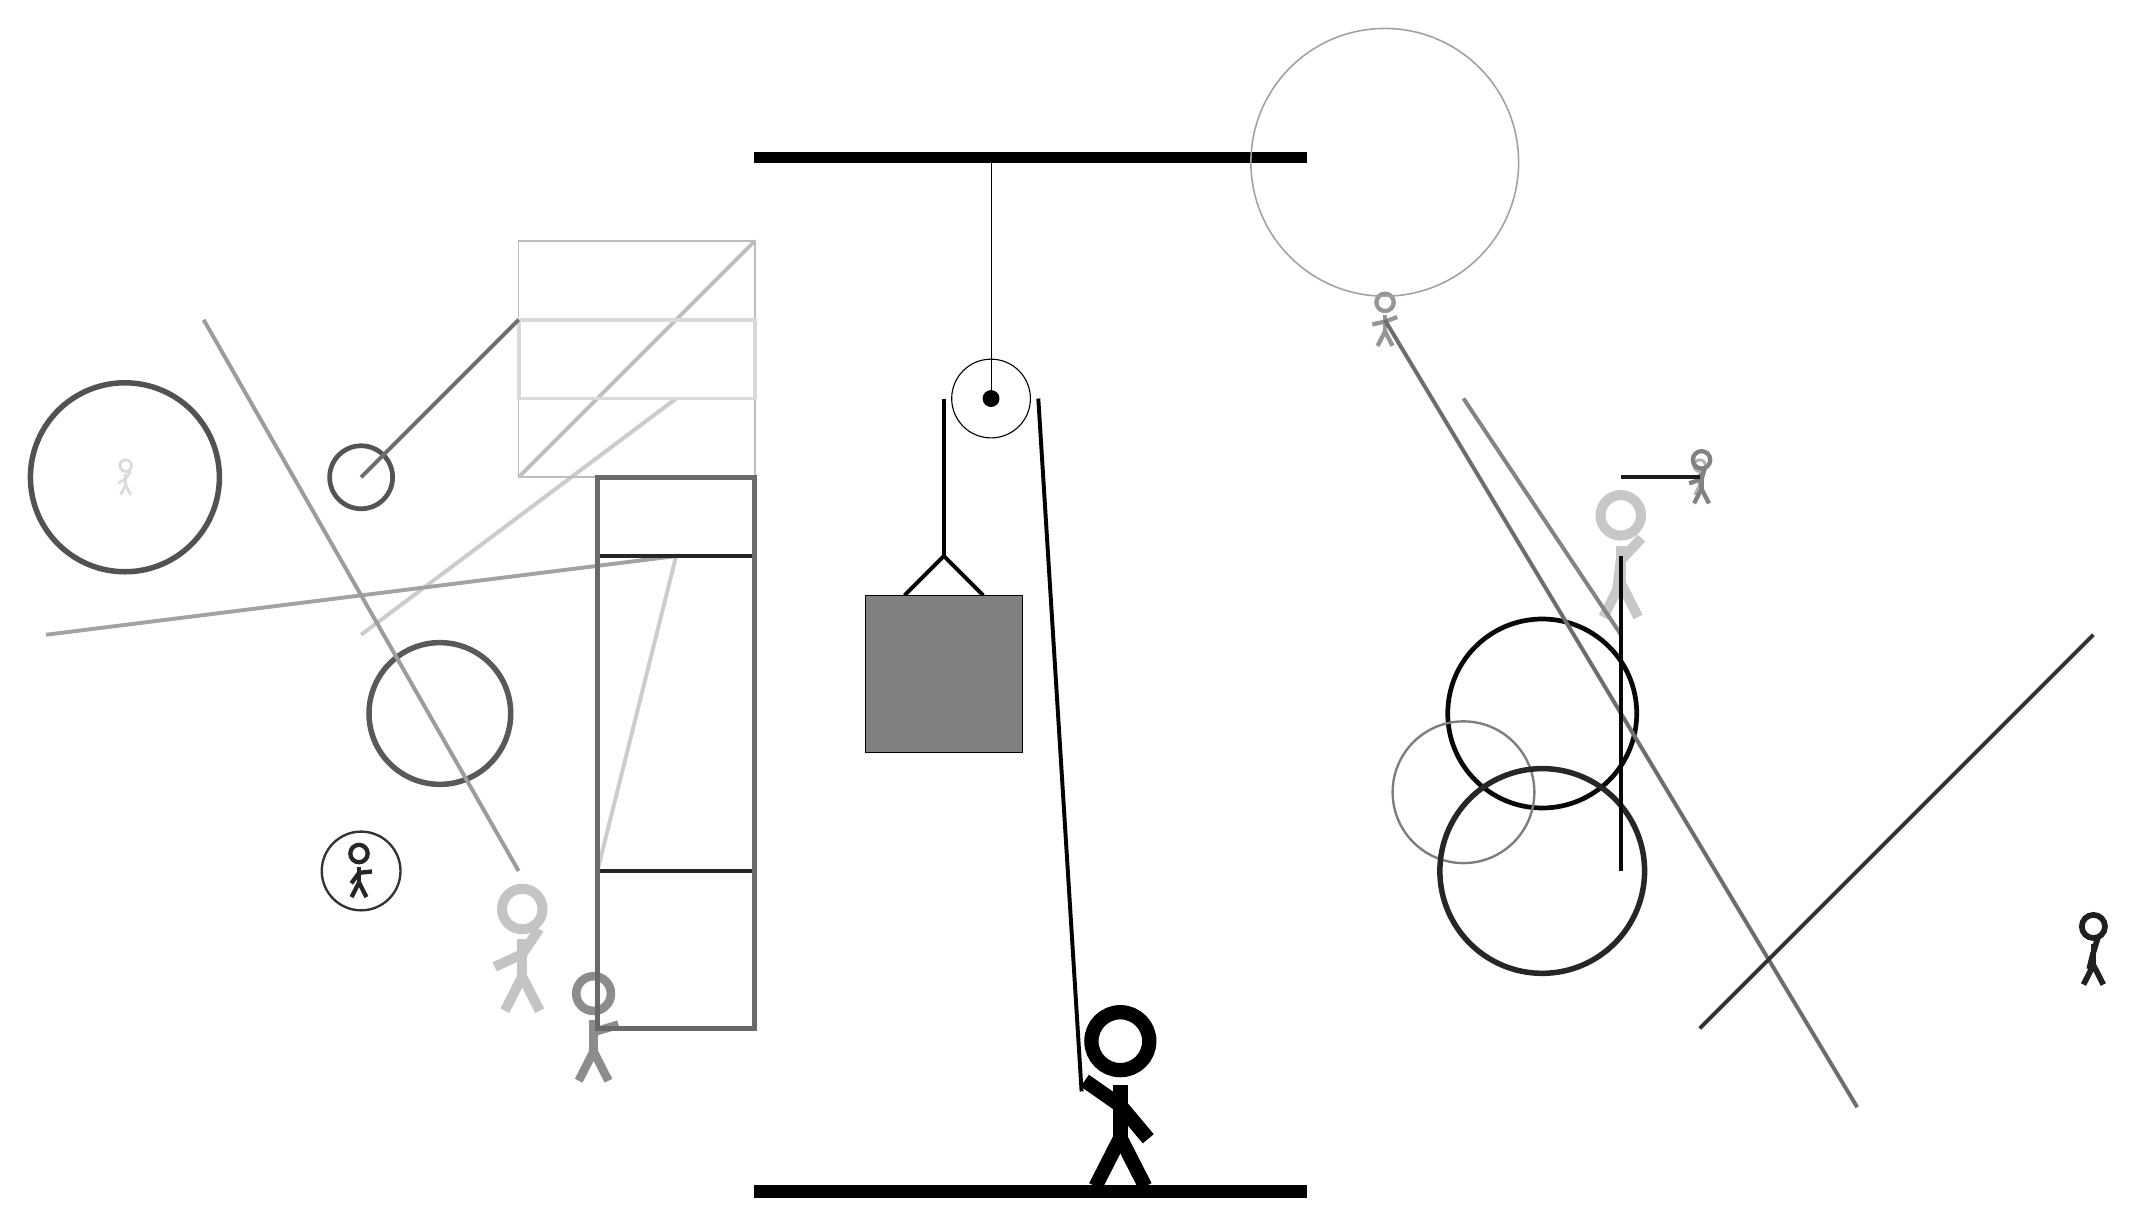
\begin{tikzpicture}
		%%%%% START %%%%%
		
		\draw[fill=black] (-2, 10) rectangle (5, 10.125);
		
		\draw (1, 7) circle (0.5);
		\draw[fill=black] (1, 7) circle (0.1);
		\draw (1, 10) -- (1, 7);
		
		\draw[line width=0.5mm] (-0.1, 4.5) -- (0.4, 5.0) -- (0.9, 4.5);
		\draw[fill=black!50] (-0.6, 4.5) rectangle (1.4, 2.5);
		
		\draw[line width=0.5mm] (0.4, 7) -- (0.4, 5.0);
		\centerarc[line width=0.5mm](1, 7)(0:180:0.6);
		\draw[line width=0.5mm](1.6, 7) -- (2.15, -1.8);
		
		\node at (2.6, -1.9) {\Strichmaxerl[10][-35][-50]};
		
		\draw [line width=0.7mm, color=black!65](-6, 3) circle (0.9);
		
		\node[line width=0.3mm, color=black!30] at (10, 6) {\Strichmaxerl[2][84][69]};
		\draw [line width=0.6mm, color=black!97](8, 3) circle (1.2);
		\node[line width=0.3mm, color=black!41] at (6, 8) {\Strichmaxerl[3][12][21]};
		\node[line width=0.4mm, color=black!14] at (-10, 6) {\Strichmaxerl[2][33][57]};
		\draw [line width=0.3mm, color=black!51](7, 2) circle (0.9);
		\draw[line width=0.5mm, color=black!20](-3, 7) -- (-7, 4);
		
		\node[line width=0.3mm, color=black!23] at (-5, 0) {\Strichmaxerl[7][25][56]};
		\draw[line width=0.5mm, color=black!36](-3, 5) -- (-11, 4);
		\draw[line width=0.2mm, color=black!26] (-2, 6) rectangle (-5, 9);
		
		\node[line width=0.7mm, color=black!88] at (15, 0) {\Strichmaxerl[4][76][73]};
		\draw[line width=0.4mm, color=black!100] (-2, -1) rectangle (-2, 5);
		\node[line width=0.5mm, color=black!49] at (10, 6) {\Strichmaxerl[3][19][73]};
		
		\draw[line width=0.5mm, color=black!57](6, 8) -- (12, -2);
		\draw [line width=0.7mm, color=black!85](8, 1) circle (1.3);
		\node[line width=0.7mm, color=black!22] at (9, 5) {\Strichmaxerl[7][83][47]};
		
		\draw[line width=0.5mm, color=black!80](10, -1) -- (15, 4);
		
		\node[line width=0.5mm, color=black!45] at (-4, -1) {\Strichmaxerl[6][89][17]};
		\draw [line width=0.2mm, color=black!37](6, 10) circle (1.7);
		\draw[line width=0.5mm, color=black!25](-5, 6) -- (-2, 9);
		\draw [line width=0.3mm, color=black!80](-7, 1) circle (0.5);
		\draw[line width=0.5mm, color=black!49](7, 7) -- (9, 4);
		\draw[line width=0.5mm, color=black!97](9, 1) -- (9, 5);
		\draw [line width=0.6mm, color=black!67](-7, 6) circle (0.4);
		\draw[line width=0.5mm, color=black!15] (-2, 7) rectangle (-5, 8);
		\draw[line width=0.5mm, color=black!39](-5, 1) -- (-9, 8);
		\draw[line width=0.5mm, color=black!89](10, 6) -- (9, 6);
		\draw[line width=0.7mm, color=black!87] (5, 1) rectangle (5, 1);
		\draw[line width=0.5mm, color=black!20](-3, 5) -- (-4, 1);
		
		\node[line width=0.3mm, color=black!85] at (-7, 1) {\Strichmaxerl[3][54][6]};
		\draw[line width=0.5mm, color=black!57](-5, 8) -- (-7, 6);
		
		\draw[line width=0.6mm, color=black!85] (-2, 5) rectangle (-4, 1);
		\draw [line width=0.7mm, color=black!68](-10, 6) circle (1.2);
		\draw[line width=0.6mm, color=black!59] (-4, 6) rectangle (-2, -1);
		
		\draw[fill=black] (-2, -3) rectangle (5, -3.15);
		
		%%%%% END %%%%%
	\end{tikzpicture}
\end{document}